\documentclass{article}

% Per-assignment macros
\def\lecturetitle{Development Environment}

% Imports
\usepackage{graphicx} % Required for inserting images
\usepackage[colorlinks=true, linkcolor=blue, urlcolor=blue, citecolor=blue, anchorcolor=blue]{hyperref}
\usepackage{hhline}

% Titling
\usepackage{titling}
\preauthor{\begin{center}}
\postauthor{\par\end{center}\vspace{-30pt}}
\setlength{\droptitle}{-50pt}

% Geometry

\usepackage{geometry}
\geometry{letterpaper, portrait, margin=1in}

\usepackage[skip=5pt]{parskip}
\newlength\tindent
\setlength{\tindent}{\parindent}
\setlength{\parindent}{0pt}
\renewcommand{\indent}{\hspace*{\tindent}}

% Assignment titling (number, due date, etc)
\title{
    Lecture Notes: \lecturetitle
}
\author{ENGR 103, Spring 2024}
\date{}

% Box environments
\usepackage{tcolorbox}
\usepackage{fancyvrb}
\newenvironment{terminalcommand}
    {\VerbatimEnvironment
    \begin{tcolorbox}[title=Terminal Command,colframe=gray!80!blue,colback=black!80!blue]
    \begin{Verbatim}[formatcom=\color{white}]}
    {\end{Verbatim}
    \end{tcolorbox}}
\newenvironment{terminaloutput}
    {\VerbatimEnvironment
    \begin{tcolorbox}[title=Terminal Output,colframe=gray!80!red,colback=black!80!blue]
    \begin{Verbatim}[formatcom=\color{white}]}
    {\end{Verbatim}
    \end{tcolorbox}}

\newenvironment{tip}
    {\begin{tcolorbox}[title=Tip,colframe=white!70!blue,colback=white]}
    {\end{tcolorbox}}

\newcounter{examplerun}
\newenvironment{examplerun}
    {\begin{tcolorbox}[title=Example Run \refstepcounter{examplerun}\theexamplerun,colframe=black!50!green,colback=white,subtitle style={boxrule=0.4pt,
colback=lightgray!80!green}]}
    {\end{tcolorbox}}
\newcommand{\exampleruninputs}{\tcbsubtitle{Inputs}}
\newcommand{\examplerunoutputs}{\tcbsubtitle{Outputs}}

\newcommand{\imagewithdefaults}[1]{\includegraphics[width=\maxwidth{0.95\columnwidth}]{#1}}

\makeatletter
\def\maxwidth#1{\ifdim\Gin@nat@width>#1 #1\else\Gin@nat@width\fi}
\makeatother

\usepackage{soul}

\begin{document}

\maketitle

Disclaimer: You don't have to use the development tools discussed below for this class. Feel free to use whatever tools you'd like. However, maintaining a working development environment is your responsibility. The TAs and I can only offer guidance when you're using tools that we're familiar with, so it's recommended that you stick with the below tools unless you're already familiar with other ones that will accomplish the same tasks.

\section{Terminals}

A \textbf{terminal} is a program that lets us interface with our computer via textual commands that get interpreted by another internal program called a \textbf{shell}. All of the software we write in this class will be text-based. That means that our programs will not create windows or tabs with graphical user interfaces. Instead, we will run our programs by issuing textual commands in a terminal, and they will output responses through text in the terminal as well. Indeed, it's difficult to write, build, and run basic software without some sort of terminal.

Luckily, all modern operating systems come with one or more terminals installed. Follow the instructions below based on your operating system to become acquainted with your terminal.

\subsection{Accessing and configuring your terminal}

\subsubsection{Windows: Powershell}

Windows actually offers a few terminals / shells. The oldest one is the Command shell (CMD). Most people consider it to be obsolete, so I don't recommend using it. The Command shell was superseded by Powershell---lots of people use this one.

To access Powershell, simply search for ``Powershell'' in the Windows start menu. When you start it, a window should appear with a text cursor. You can now begin issuing textual commands to your computer by typing them and pressing enter. We'll learn about some commands shortly.

When you open Powershell for the first time, it will default to a certain configuration that most people don't like, so you may want to do some reconfiguration. If you right click on the window's menu bar (the top of the window) and click ``Properties'', you can configure your terminal to your liking (e.g., background colors, font colors, font sizes, etc):

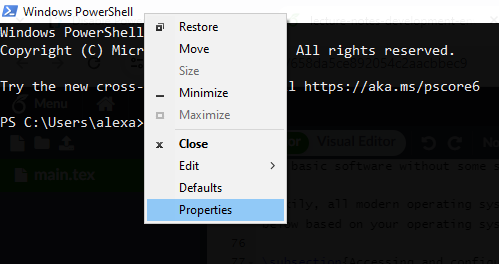
\includegraphics[width=\maxwidth{0.95\columnwidth}]{res/properties.PNG}

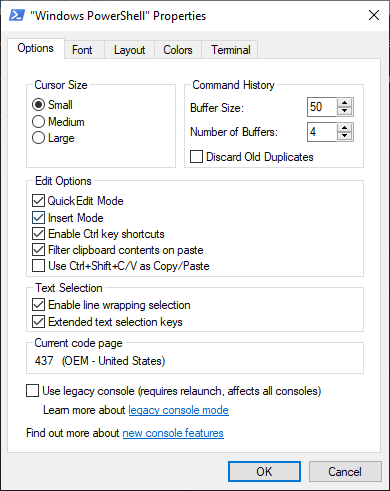
\includegraphics[width=\maxwidth{0.95\columnwidth}]{res/properties-window.PNG}

\subsubsection{Mac: ``Terminal''}

Mac comes with a terminal by default. It's simply called ``Terminal'', and you can find it by typing ``Terminal'' into the Mac Spotlight search (the magnifying glass at the topright corner of your screen).

When you open your Mac Terminal for the first time, it will default to a certain configuration that most people don't like, so you may want to do some reconfiguration. In the menu bar, navigate to Terminal $\rightarrow$ Preferences, then navigate to the Profiles tab. From here, you can add new terminal profiles and modify existing ones. A profile is basically just a configuration of terminal settings. For most cases, it's sufficient to just modify the default profile (e.g., ``Basic''). You can change default font sizes, colors, etc.

\subsubsection{*nix: Whatever terminal you want}

If you're running a *nix OS other than Mac (e.g., Linux, FreeBSD, etc), then you probably already know what a terminal is. Most *nix terminals are extremely similar since the default shell is configured at a user level, so use whatever terminal you want.

\section{ENGR Servers}

In some sense, you can think of a terminal as being similar to the Windows File Explorer or Mac Finder, but everything is text-based. By issuing textual commands in your terminal (i.e., typing them and pressing enter), you can navigate your file system, view files, edit files, and execute files (if they're executable). Indeed, anything you can do in a file explorer, you can also do in a terminal. But there are also lots of things that you can do in a terminal that you can't do in a file explorer. For this reason, terminals are indispensable tools when you need to interface with your computer in intricate ways, such as in software development.

However, we're going to do things a little differently in this course. Rather than issuing commands to \textit{our} computer via the terminal, we're primarily going to be issuing commands to a different computer. In particular, OSU's College of Engineering has some big, fancy computers in the Kelley Engineering Center's server room. I'll refer to these computers as the \textbf{ENGR servers}. For this course, we're going to be doing all of our work on the ENGR servers. But there's one issue---the ENGR servers don't have monitors, mice, or keyboards attached to them (not to mention, they're behind locked doors, and only certain faculty and staff are allowed physical access). So... How do we use them?

Well, it's simple---we're going to issue a single command to \textit{our} computer's terminal to instruct our computer to connect to the ENGR servers remotely. At that point, we will be able to control the ENGR servers via a remote shell (i.e., we will be able to type commands into \textit{our} terminal to control the ENGR servers). Note that this requires internet access.

Of course, connecting to and controlling OSU's ENGR servers requires authentication. First, you have to create an ENGR account if you don't already have one. To do this, navigate to \href{https://teach.engr.oregonstate.edu/teach.php?type=want_auth}{CoE TEACH}, click ``Create a new account'', and follow the instructions on screen to create your ENGR account.

Once you have an ENGR account setup, you should be able to connect to the ENGR servers from your terminal. To do this, type the following command into your terminal and press enter, substituting \texttt{<ONID>} with your ONID (e.g., mine is ``guyera''):

\begin{terminalcommand}
    ssh <ONID>@access.engr.oregonstate.edu
\end{terminalcommand}
\texttt{ssh} stands for ``Secure Shell''. It is a cryptographic network protocol that lets you connect to and control another computer remotely with a predefined user account and associated permissions.

At this point, your terminal should prompt you for a password (if not, then there's likely something wrong with your internet connection, or perhaps the ENGR servers are temporarily down). Type in your ONID password and press enter (i.e., the password you use to login to OSU services, like Canvas and Outlook). \underline{Note that your password will be invisible as you type it}. That's okay---it's an intended security feature.

Your terminal should now prompt you to verify your login via Duo. If you have multiple Duo devices, then it will ask you which duo device you'd like to use for authentication. My terminal prompt looks like this:

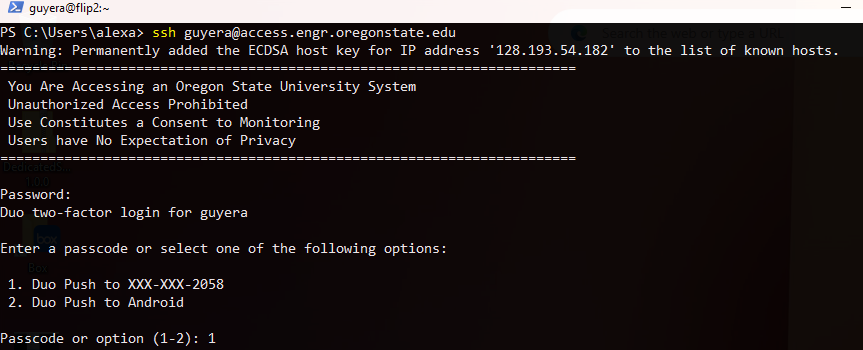
\includegraphics[width=\maxwidth{0.95\columnwidth}]{res/login-start.PNG}

Type the desired device number and press enter. Approve the Duo push via your device.

You should now be logged into the ENGR servers. My terminal prompt looks like this:

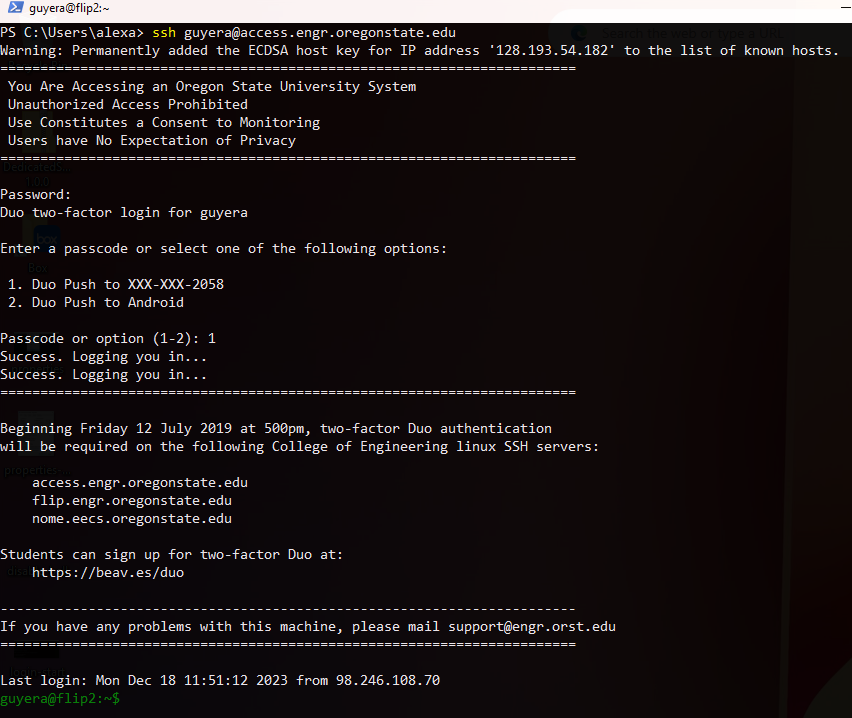
\includegraphics[width=\maxwidth{0.95\columnwidth}]{res/login.PNG}

The ENGR servers run Linux, which means any commands you type into your terminal from here on out will be interpreted by the ENGR servers as Linux shell commands. You can configure your user account's Linux shell on TEACH, but the default one will work just fine. In addition, it's important to understand that, since your terminal is now controlling the ENGR servers rather than your own computer, you are now operating on the ENGR filespace. Soon, we will learn how to create and edit files on the ENGR server---understand that these files will be located on the ENGR servers and cannot be accessed trivially from your computer / Windows File Explorer / Mac Finder (if you wanted to transfer files between your computer and the ENGR servers, you'd have to use a file transfer protocol like SFTP or SCP; feel free to Google it).

Some terminology: When we say something is \textbf{local}, or done \textbf{locally}, it means that it occurs directly on your computer. When we say something is \textbf{remote}, or done \textbf{remotely}, it means that it occurs on the ENGR servers (or whatever server you're connected to).

\section{Linux shell commands}

Now that our terminal is connected to the ENGR servers, we should learn how to use it. To summarize, here is a table briefly describing some important *nix shell commands:

\begin{tabular}{|p{0.3\columnwidth}|p{0.65\columnwidth}|}
    \hline
    Command & Description\\
    \hline
    \texttt{ssh <connection string>} & Connects to the SSH server specified by the connection string. You already used this command locally (from your computer) to connect to the ENGR servers.\\
    \hline
    \texttt{pwd} & Prints the working directory\\
    \hline
    \texttt{ls <path>} & Lists the files and directories within directory located at the specified path\\
    \hline
    \texttt{ls} & Lists the files and directories within the working directory\\
    \hline
    \texttt{mkdir <path>} & Creates a new directory at the specified path\\
    \hline
    \texttt{cd <path>} & Navigates to the directory at the specified path, making it the new working directory\\
    \hline
    \texttt{cd} & Navigates to your home directory, making it the new working directory (on the ENGR servers, this should be \texttt{/nfs/stak/<ONID>})\\
    \hline
    \texttt{clear} & Clears the text on-screen in the terminal\\
    \hline
    \texttt{cp <path1> <path2>} & Copies the file located at the specified path1 to the location specified by path2. \texttt{cp -r <path1> <path2>} can be used to copy an entire directory and all of its contents.\\
    \hline
    \texttt{mv <path1> <path2>} & Moves the file or directory located at the specified path1 to the location specified by path2. This can also be used to rename files / directories. If the specified path2 already exists and is itself a directory, this will move the file / directory located at the specified path1 \textit{into} the directory located at the specified path2.\\
    \hline
    \texttt{rm <path>} & Removes (deletes) the file located at the specified path. To remove an entire non-empty directory, use \texttt{rm -r <path>}. To remove an empty directory, you can also use \texttt{rmdir <path>}.\\
    \hline
    \texttt{cat <path1> <path2> ... <pathN>} & Concatenates the contents of the files at all of the specified paths in the order provided and prints the concatenated content to the terminal. Note that this is also used for just printing the contents of a single file.\\
    \hline
    \texttt{vim <path>} & Opens the file at the specified path in the vim text editor (see next section)\\
    \hline
\end{tabular}

Let's talk about those commands in some more detail.

As I mentioned, you can think of your terminal like a file explorer, but text-based. At any given point in time, your terminal / shell is ``located'' in a certain folder. In the context of terminals, we tend to refer to folders more rigorously as \textbf{directories}. At any given point, the directory that your terminal is currently operating in is referred to as the \textbf{working directory}. To check your working directory, execute the following command:

\begin{terminalcommand}
    pwd
\end{terminalcommand}

\texttt{pwd} stands for ``print working directory''. To \textbf{print} means to display some text to the terminal. The output might look something like this:

\imagewithdefaults{res/pwd-output.png}

Notice that, after logging in, my working directory is \texttt{/nfs/stak/users/guyera} by default. This is referred to as my \textbf{home directory} on the ENGR servers. All ssh sessions will start out in the home directory. Yours will look similar, but my ONID will be replaced with yours.

Of course, directories can have other files and directories inside them. To list the files and directories that reside in your working directory, run the following command:

\begin{terminalcommand}
    ls
\end{terminalcommand}

\texttt{ls} stands for ``list''. The output might look something like this:

\imagewithdefaults{res/ls-output.png}

Notice that the outputs are colored. Yours are probably colored as well, but the colors themselves may be different. In my case, directory names are colored blue, symbolic links are colored light blue (we won't talk about these), and files are colored differently according to their permissions.

Before moving on, let's talk about paths. A \textbf{path} is a string (i.e., a sequence of characters) that represents the location of a file or directory. Directories in a path are separated by some sort of path separator. On *nix systems (including Linux, which the ENGR servers run), a forward slash (\texttt{/}) is used as the path separator. For example, if a directory \texttt{A} contains another directory \texttt{B} which contains an image file \texttt{C.jpg}, the path of the image file might be something like \texttt{A/B/C.jpg}.

Paths come in two forms: absolute and relative. A \textbf{relative path} is the location of a file or directory \underline{relative to the working directory}. In this course, you'll mostly be working with relative paths. For example, \texttt{A/B/C.jpg} is a relative path---it refers to the image file called \texttt{C.jpg}, which resides within directory \texttt{B}, which resides within directory \texttt{A}, \underline{which resides within the working directory}. If directory \texttt{A} doesn't reside within the working directory (or directory \texttt{B} doesn't reside within directory \texttt{A}, or file \texttt{C.jpg} doesn't reside within directory \texttt{B}), then the path points to a nonexistent file.

An \textbf{absolute path} is the location of a file or directory within the entire system. On *nix systems, an absolute path starts with a path separator (\texttt{/}). For example, \texttt{/nfs/stak/users/guyera/A/B/C.jpg} is an absolute path---it refers to the location of \texttt{C.jpg} within the entire file system. Note that absolute paths are useful when you need to represent the location of a file or directory that works from anywhere (i.e., points to the same location regardless of the working directory). However, the downside is that absolute paths aren't very portable because they assume a particular directory structure for the entire file system.

Residing within every directory, there are two implied directories: ``\texttt{.}'' and ``\texttt{..}''. The former (\texttt{.}) refers to the containing directory itself. For example, \texttt{A/.} is the same thing as \texttt{A} (they're both paths that point to directory \texttt{A}). The latter (\texttt{..}) refers to the \textbf{parent directory} (i.e., the directory that contains the containing directory). For example, \texttt{A/B/..} is the same thing as \texttt{A} because \texttt{A/B/..} refers to the directory that contains \texttt{B} (i.e., the parent directory of \texttt{B}), which is directory \texttt{A}. These will be important later on.

There is also a special path that denotes your home directory---a simple tilde ($\sim$). For example, \texttt{$\sim$/A} refers to the file / directory called \texttt{A} that resides within your home directory. In my case, \texttt{$\sim$/A} is equivalent to \texttt{/nfs/stak/users/guyera/A} when I'm on the ENGR servers.

Lastly, any path that points to a directory can optionally end with a trailing path separator (\texttt{/}). This doesn't change the semantics of the path. For example, \texttt{$\sim$/A/B/} is equivalent to \texttt{$\sim$/A/B}.

Paths are very useful. Any time you need to issue a shell command that operates on a file, you specify the file via a path (relative or absolute). For example, in addition to using \texttt{ls} to list the files and directories that reside within the working directory, you can also use it to list the files and directories that reside in some other directory, like so:

\begin{terminalcommand}
    ls <path>
\end{terminalcommand}

In this command, \texttt{<path>} is referred to as a \textbf{command line argument}. In general, \textbf{arguments} are inputs to computational procedures or functions. In this case, this will list the files and directories that are contained within the directory specified by the given path. For example, \texttt{ls A} would list the files and directories that reside within directory \texttt{A}, which in turn resides within the working directory.

Of course, just listing information about a file system isn't very useful. We want to be able to create new directories, navigate directories, write new files, and read / print existing ones all via shell commands. Let's start with creating new directories. To create a new directory, run the following command:

\begin{terminalcommand}
    mkdir <path>
\end{terminalcommand}

This creates the directory at the location specified by the path. It will fail if the directory already exists or if you don't have the necessary permissions to create the directory. It will also fail if the directories \textit{along} the path don't already exists. For example, \texttt{mkdir A/B} will fail if directory \texttt{A} doesn't already exist. If you want to create a directory along with all of its ancestors within a path as necessary, you can supply the \texttt{-p} flag, like so:

\begin{terminalcommand}
    mkdir -p <path>
\end{terminalcommand}

Let's see it in action:

\imagewithdefaults{res/mkdir-p.png}

Here, I used \texttt{mkdir} with the \texttt{-p} flag to create an \texttt{engr103} directory within my home directory, as well as a \texttt{lecture-notes} directory within the \texttt{engr103} directory, all in one command. I then proceeded to list the contents of the \texttt{engr103} directory to prove that everything worked as expected.

Next, to navigate from one directory to another (i.e., to change our working directory, or the directory that our terminal / shell is currently operating in), we can use the following command:

\begin{terminalcommand}
    cd <path>
\end{terminalcommand}

\texttt{cd} stands for ``change directory'', and it does just that---it changes your working directory to the one located at the specified path. For example:

\imagewithdefaults{res/cd.png}

You can also use \texttt{cd} with no command line arguments:

\begin{terminalcommand}
    cd
\end{terminalcommand}

This will change your working directory back to your home directory. For example:

\imagewithdefaults{res/cd-home.png}

As you run lots of terminal commands, your terminal output will become very cluttered. You can clear the contents of the terminal via the following command:

\begin{terminalcommand}
    clear
\end{terminalcommand}

Notably, when your shell interprets the \texttt{clear} command, it will send a hint to your terminal to clear its screen. The terminal is responsible for doing the actual clearing. This means that different terminals might interpret the \texttt{clear} command differently, even when connected to the same ENGR servers via SSH. On some terminals, it may just clear the screen by scrolling down a bunch, allowing you to scroll back up to see the old text. On other terminals, it will actually remove the old text from the presentation buffer, so you can't scroll up and see it anymore. On some terminals, running \texttt{clear} once will scroll down, and running it twice (in a row) will clear the buffer. You should play around with your terminal and get acquainted with its behavior---clearing your terminal's buffer is often very helpful when you need a clean presentation (e.g., of compilation errors for debugging).

Next, you can copy a file via the following command:

\begin{terminalcommand}
    cp <path1> <path2>
\end{terminalcommand}

This will copy the file located at the specified path1 to the location specified by path2. If path2 already exists and is itself a directory, this will copy the file at path1 \textit{into} the directory at path2.

Note that this only works for copying \textit{files}. If you want to copy an entire directory and all of its contents, you have to supply the \texttt{-r} flag:

\begin{terminalcommand}
    cp -r <path1> <path2>
\end{terminalcommand}

It works the same, but it works for directories as well.

If you just want to \textit{move} a file or directory without copying it, you can use the \texttt{mv} command:

\begin{terminalcommand}
    mv <path1> <path2>
\end{terminalcommand}

It behaves very similarly to \texttt{cp}, except it simply moves the file / directory from one place to another rather than creating a copy of it at the new location. Note that the \texttt{mv} command works on both files and directories---no need to supply at \texttt{-r} flag to move directories. Unsurprisingly, though perhaps not so intuitively, you can use the \texttt{mv} command to rename a file---just think of it as ``moving'' the file from its original path (including its old name) to a new path (including its new name).

Lastly, you can remove files using the \texttt{rm} command:

\begin{terminalcommand}
    rm <path>
\end{terminalcommand}

This removes the file at the location specified by the path. Note that \texttt{rm} behaves similarly to \texttt{cp}---it only works on files. If you want to remove an entire directory and all of its contents, you have to supply the \texttt{-r} flag:

\begin{terminalcommand}
    rm -r <path>
\end{terminalcommand}

\section{vim}

By this point, you should know most of everything you need to know about navigating a file system in a terminal. The next step is to learn how to create and edit new text-based files directly within a terminal. To do that, we need a terminal-based text editor (i.e., a text editor that runs directly within our terminal rather than within a separate window like notepad or Microsoft Word). There are a few options available to you on the ENGR servers, including \texttt{vim}, \texttt{nano}, and \texttt{emacs}. We'll use \textbf{vim} for this course.

To open a file in vim, run the following command:

\begin{terminalcommand}
    vim <path>
\end{terminalcommand}

This will open the file located at the specified path in vim \underline{even if the file doesn't currently exist} (if it doesn't exist, it will be created). For example, suppose we want to create a file called \texttt{hello.txt} in our working directory. Then we might run \texttt{vim hello.txt}.

vim is a text editor, similar to notepad or Microsoft Word. However, because it's entirely terminal-based (and terminals are entirely text-based), there are no menu buttons anywhere! For example, your terminal might look a bit like this after opening \texttt{hello.txt} as above:

\imagewithdefaults{res/vim-open.png}

Yours will probably be slightly different (e.g., it won't have line numbers), but it'll be pretty similar. It looks like there's a menu at the top, but that's my terminal menu---not a vim menu. Indeed, if we want to save our text file, quit, or even copy and paste text within vim, we have to do so through text-based \textbf{vim commands}.

For this reason, vim operates in one of several \textbf{vim modes}. By default, vim starts up in \textbf{normal mode}. Normal mode is used for issuing commands, like saving the text file, quitting vim, copying and pasting, and so on. If you want to actually write text into the file, you have to switch to \textbf{insert mode}. To switch from normal mode to insert mode, press the \texttt{i} key. From here, you can start writing text into your text file. Let's write ``Hello, world!'':

\imagewithdefaults{res/vim-text.png}

\begin{tip}
Note that lots of vim hotkeys and commands are case-sensitive, though lowercase \texttt{i} and uppercase \texttt{I} should both work for switching to insert mode. In any case, make sure your caps lock is turned off as appropriate when running vim commands and hotkeys, or you'll run into a lot of headache.
\end{tip}

Now, let's save our text file and quit. However, as mentioned, saving and quitting requires issuing vim commands because there are no menu buttons. We're currently in insert mode, and you can't issue vim commands from insert mode. First, we have to switch back to normal mode. To do this, press the escape key.

Now, to issue a command from normal mode, start by typing a colon (\texttt{:}). The colon should appear at the bottom-left of your screen, like so:

\imagewithdefaults{res/vim-command.png}

Following the colon, type the \textbf{vim command} that you want to execute. Here is a table of a few basic vim commands (there are \textit{lots} of cool vim commands that we don't have time to cover in this course [e.g., find and replace]---I encourage you to further acquaint yourself with your development tools in your own time):

\begin{tabular}{|p{0.3\columnwidth}|p{0.65\columnwidth}|}
    \hline
    Command & Description\\
    \hline
    \texttt{w} & Write (save) the file\\
    \hline
    \texttt{q} & Quit vim (without saving)\\
    \hline
    \texttt{wq} & Write (save) the file and quit\\
    \hline
    \texttt{set mouse=a} & Enable the mouse in vim (it's disabled by default)\\
    \hline
    \texttt{set nu} & Display line numbers\\
    \hline
    \texttt{syntax on} & Enable syntax highlighting (usually enabled by default, but may need to be enabled in certain circumstances)\\
    \hline
    \texttt{colorscheme <colorscheme>} & Set the syntax highlighting colorscheme. Writing \texttt{:colorscheme } and pressing tab should cycle you through the available options.\\
    \hline
\end{tabular}

In this case, we want to save and quit. So we'll execute the \texttt{wq} command. After the colon, type \texttt{wq} and press enter, like so:

\imagewithdefaults{res/vim-wq.png}

This should bring you back to your regular ssh session.

\begin{tip}
You can create a file called \texttt{.vimrc} in your home directory (e.g., by opening and editing it via \texttt{vim $\sim$/.vimrc}) and fill it with a bunch of vim commands (without the colons, and each command going on their own line). These commands will be executed by default whenever you open vim. This is useful for enabling things like line numbers and the mouse by default.
\end{tip}

If we run \texttt{ls}, we can see that \texttt{hello.txt} is now present in our working directory:

\imagewithdefaults{res/ls-hello.png}

Great! Lastly, let's learn one more terminal command: \texttt{cat}. The \texttt{cat} command stands for ``concatenate'', and it was originally designed for concatenating the contents of files together, like so:

\begin{terminalcommand}
    cat <path1> <path2> ... <pathN>
\end{terminalcommand}

This concatenates the contents of the files at all of the specified paths in the provided order and prints the concatenated content to the terminal. However, you can also run the \texttt{cat} command on just a single file path. Indeed, this is how you print the contents of a file to the terminal. For example, running \texttt{cat hello.txt} will print the contents of \texttt{hello.txt} to the terminal:

\imagewithdefaults{res/cat.png}

\section{Git}

Suppose you've been working on a large program for weeks. You've completed 90\% of the work, and everything seems to be functioning properly---there's just a few small changes left to make. You complete those changes, and... Uh oh! Everything that was once functioning properly is now broken. The deadline is swiftly approaching, and you have nothing to deliver...

Indeed, code can be very delicate (especially if you don't have the know-how to write more robust code). In order to avoid the above problem, it's a good idea to frequently save snapshots (backups) of working (and non-working) versions of your code. There are tools called \textbf{V}ersion \textbf{C}ontrol \textbf{S}ystems (VCS) that help us do exactly this (and more!). The most popular VCS is called \textbf{Git}.

As mentioned, Git helps you save \textbf{snapshots}, also called \textbf{commits}, of your code at any given point in time. In fact, it can be used to save commits of any kind of digital project, though software engineers tend to use it the most. It stores these commits via a technique called delta compression, which makes it very space-efficient when only small changes are made between commits.

Git is a \textbf{command-line utility}, which means that we interact with it via a terminal. Git is pre-installed on the ENGR servers, so you can use it so long as you're connected to them via SSH. Of course, you can also install Git on your own computer.

Before using Git in any way, you should start by configuring your global Git parameters. In particular, you should inform Git of your name and email address; Git will store this information along with any commits that you create for any project while working on the ENGR servers (you can change these parameters at any time, and you can also override them with local parameters). To do this, run the following commands:

\begin{terminalcommand}
git config --global user.name "<Your name>"
git config --global user.email "<Your email>"
\end{terminalcommand}

Replace \texttt{<Your name>} and \texttt{<Your email>} with your full name and email address, respectively.

You're now ready to use Git. Git works by keeping track of so-called ``repositories'', also called ``repos'' for short. A Git repo is simply a tagged directory containing the work associated with a digital project (e.g., a folder containing some source code files for some software).

There are two main ways to create a Git repo and start using Git:

\begin{enumerate}
    \item \label{item:remote_to_local} Create a Git repo on a Git repo-hosting site. Like most people, we'll use GitHub as our repo-hosting site. Then, ``clone'' (copy) that repo into your filespace (e.g., your computer, or your filespace on the ENGR servers) via the \texttt{git clone} command. This will create a new directory in your working directory that's been tagged as a Git repo, contains all of the files associated with the cloned repo on GitHub, and is set up to ``track'' the cloned repo on GitHub (so that you sync your local repo's files with the GitHub repo's files).
    \item Tag an existing directory in your filespace as a Git repo via the \texttt{git init} terminal command. From here, you can optionally configure this local Git repo to track a remote repo (e.g., one on GitHub).
\end{enumerate}

We'll be using method \ref{item:remote_to_local} in this course.

Once you have an account on GitHub, the process to create a repo through the web interface is fairly straightforward. Once you've created a repo on GitHub or via GitHub Classroom (or have access to someone else's repo, such as \href{https://github.com/chromium/chromium}{this one}), you can clone it onto your computer / ENGR file space by executing the following terminal command:

\begin{verbatim}
git clone <SSH URL OF GITHUB REPO>
\end{verbatim}

Replace \texttt{<SSH URL OF GITHUB REPO>} with the SSH URL of the GitHub repo that you want to copy (clone) into your filespace. A GitHub repo's SSH URL can be found on the repo's page by clicking on the green ``\texttt{<> Code}'' button, and then clicking on the ``SSH'' tab. Note: You can only clone a repo if you have the necessary permissions. During your week 2 studio, you'll learn how to setup these permissions and how to authenticate with GitHub from the ENGR servers using SSH keys. If you want to follow along with these lecture notes on your own repo, you should go complete the setup portion of the week 2 studio before continuing.

At this point, if you execute \texttt{ls}, you should now see a new directory in your working directory whose name is similar to that of the GitHub repo that you just cloned. If you enter that directory via \texttt{cd} and run \texttt{ls} again, you'll see that it contains all of the same files as the GitHub repo.

When your working directory (or any of the working directory's ancestors) is tagged as a Git repo, you can execute various \texttt{git} commands to operate on the repo. For example, you can see the status of the Git repo by executing the following command:

\begin{terminalcommand}
git status
\end{terminalcommand}

Note that the above command, along with all other git commands, will only work if your working directory (or one of its ancestors) is part of a Git repo.

Suppose I've just cloned a repo that has a single file in it called \texttt{main.cpp}, which contains the following C++ source code:

\begin{verbatim}
#include <iostream>

int main() {
    std::cout << "Hello, World!" << std::endl;
}
\end{verbatim}

Assuming I haven't modified this file or created any new files in the repo since I cloned it, if I execute \texttt{git status}, the output will look something like this:

\imagewithdefaults{res/fresh-git-status.png}

There's a few things to unpack here. Firstly, the output says ``On branch main''. We won't talk much about Git branches in this course, but they effectively represent alternative versions of your repo which can be merged together into a final repo. The main purpose of branches is to facilitate teamwork on a large project. For this course, you'll always be working on a single ``main'' branch to keep things simple, so you don't really have to think about branches that much.

Next, the output says ``Your branch is up to date with `origin/main'.'' This simply means that we haven't created any new commits yet that need to be synced back up with the repo on GitHub (i.e., our local repo is not ahead of the GitHub repo from which it was cloned).

Lastly, the output says ``nothing to commit''. This simply means that we haven't made any changes to any of the files in the repo since we cloned it, or since we last created a commit, and so there would be no purpose in creating a new commit at this point (in fact, Git won't even let you create a new commit if you haven't modified and staged any files since the last commit).

Suppose, however, that we modify \texttt{main.cpp}, removing the semicolon after \texttt{std::endl}:

\clearpage

\begin{verbatim}
#include <iostream>

int main() {
    std::cout << "Hello, World!" << std::endl;
}
\end{verbatim}

If we execute \texttt{git status} again, the output will look something like this:

\imagewithdefaults{res/git-status-modified.png}

Notice: Under ``Changes not staged for commit'', it lists \texttt{main.cpp}. This means that \texttt{main.cpp} has been modified since the last commit.

In general, each file in a Git repo falls into one of three categories:
\begin{enumerate}
    \item Modified
    \item Staged
    \item Committed
\end{enumerate}

\textbf{Modified} files are files that have been changed since the last commit in which they were included, or new files that have never been included in any commits (i.e., ``untracked'' files). \textbf{Staged} files are files that are prepared to be stored in the next commit. \textbf{Committed} files are files that have \ul{not} been changed since they were last stored in a commit.

Indeed, when you want to create a new commit, you first have to decide which files' changes (i.e., latest versions) should be reflected in that commit. We do this by \textbf{staging} them using the \texttt{git add} command:

\begin{terminalcommand}
git add <file1> <file2> ... <fileN>
\end{terminalcommand}

You can also stage entire directories. In fact, if you want to stage every file in your entire repo, you could just stage the entire repo directory itself.

Suppose we want to create a commit of our repo that includes the latest version of \texttt{main.cpp} (with the semicolon removed). Then we'd first have to stage \texttt{main.cpp} via:

\begin{verbatim}
git add main.cpp
\end{verbatim}

After that, running \texttt{git status} again will output something like this:

\imagewithdefaults{res/git-status-staged.png}

Notice that \texttt{main.cpp} is now listed as a ``change to be committed''---it's staged for the next commit.

When you're done staging your next commit, you can create the commit itself by executing the following command:

\begin{terminalcommand}
git commit -m "<Commit message>"
\end{terminalcommand}

Replace \texttt{<Commit message>} with a brief note explaining the changes that were made relative to the previous commit. As a rule of thumb, you should prefer to create new commits \ul{very frequently} with just a few, small changes between them, so your commit messages should only need to be one or two sentences.

Suppose that I want to commit my changes to \texttt{main.cpp}. Then I might do something like this:

\begin{terminalcommand}
git commit -m "Remove semicolon after std::endl"
\end{terminalcommand}

After running the above command, let's run \texttt{git status} again. It now outputs the following:

\imagewithdefaults{res/git-status-commit.png}

Notice: there are no more modified or staged files. Everything is committed. However, it says ``Your branch is ahead of `origin/main' by 1 commit.'' This is telling us that we've created a new commit in our local repo (on our filesystem), but we haven't synced that new commit with the remote repo that we cloned from GitHub. Indeed, if we opened up our GitHub repository's page at this point, it would be outdated---its version of \texttt{main.cpp} would still include the semicolon.

To fix this synchronization issue, we need to upload, or \textbf{push}, our new commit(s) to our GitHub repo. To push commits that you've created in a local repo to the remote repo that it's set up to track, execute the following command:

\begin{verbatim}
git push
\end{verbatim}

Assuming you created your local repo by cloning a remote repo, this should work out-of-the-box. In other cases (e.g., if you created your local repo via \texttt{git init}), this may require some additional configuration beforehand. Regardless, this command will only succeed if you have the proper permissions to push changes to the remote repo from your shell. Again, you'll learn how to set up these permissions for your own GitHub repos via SSH keys in the week 2 studio.

If I execute the above command and run \texttt{git status} again, the output now looks like this:

\imagewithdefaults{res/git-status-push.png}

Our repo status is back to where it started. All changes have been committed, and all commits have been uploaded to GitHub. At this point, if we navigate back to our GitHub repository in a browser and refresh the page, we'll see that \texttt{main.cpp} has been updated, and the semicolon has been removed.

Let's cover just a couple more useful Git commands. Firstly, you can view the history of commits in your Git repo via the following command:

\begin{terminalcommand}
git log
\end{terminalcommand}

Running this command right now will output something like the following:

\imagewithdefaults{res/git-log.png}

For each commit in reverse-chronological order, it will list the commit's hash (the long string of seemingly random characters in the above screenshot, which is used to identify the commit), author, timestamp, and message. There are two commits here. The first one (with message ``Init'') was present in the GitHub repo before I even cloned it (I created it ``off-screen'', and it simply initialized the repository with the first version of \texttt{main.cpp}). The second one is the one that we just created in which we removed the semicolon after \texttt{std::endl}.

Suppose you have a modified (unstaged) file in your repo. In such a case, you can view the changes that have been made to that file since the last commit in which it was included via the following command:

\begin{terminalcommand}
git diff <file>
\end{terminalcommand}

For example, if I add the semicolon back to \texttt{main.cpp}, and then I execute \texttt{git diff main.cpp} (without staging or committing my changes), it will output something like the following:

\imagewithdefaults{res/git-diff.png}

\texttt{git diff} displays changes in terms of lines removed and lines added. In this case, it shows that I removed one line of code (in red, prefixed with a minus sign) and replaced it with another (in green, prefixed with a plus sign). The only actual change is the insertion of the semicolon at the end.

Suppose I stage and commit my changes to \texttt{main.cpp}. Running \texttt{git log} again will now show three commits:

\imagewithdefaults{res/git-log-two.png}

There are many other useful Git commands. In fact, I said that one of the main purposes of VCS is to save snapshots of your work so that you can rollback to previous versions in case you accidentally implement a breaking change. Of course, there's a Git command that will let you do that: \texttt{git revert} (there's also \texttt{git reset}, but it's more destructive and generally harder to use correctly than \texttt{git revert}). There are many other Git commands as well, such as \texttt{git pull}, \texttt{git branch}, \texttt{git merge}, \texttt{git rebase}, and so on. We don't have time to cover all of them, so we've focused on the ones that you'll need to be successful in this course. Feel free to study some of these other commands on your own or ask about them outside of class.

\end{document}
